\subsection{Facebooks end-to-end kommunikations chathoved}
\label{appendix:facebookchat}
\begin{figure}[H]
    \begin{subfigure}{0.33\textwidth}
        \centering
        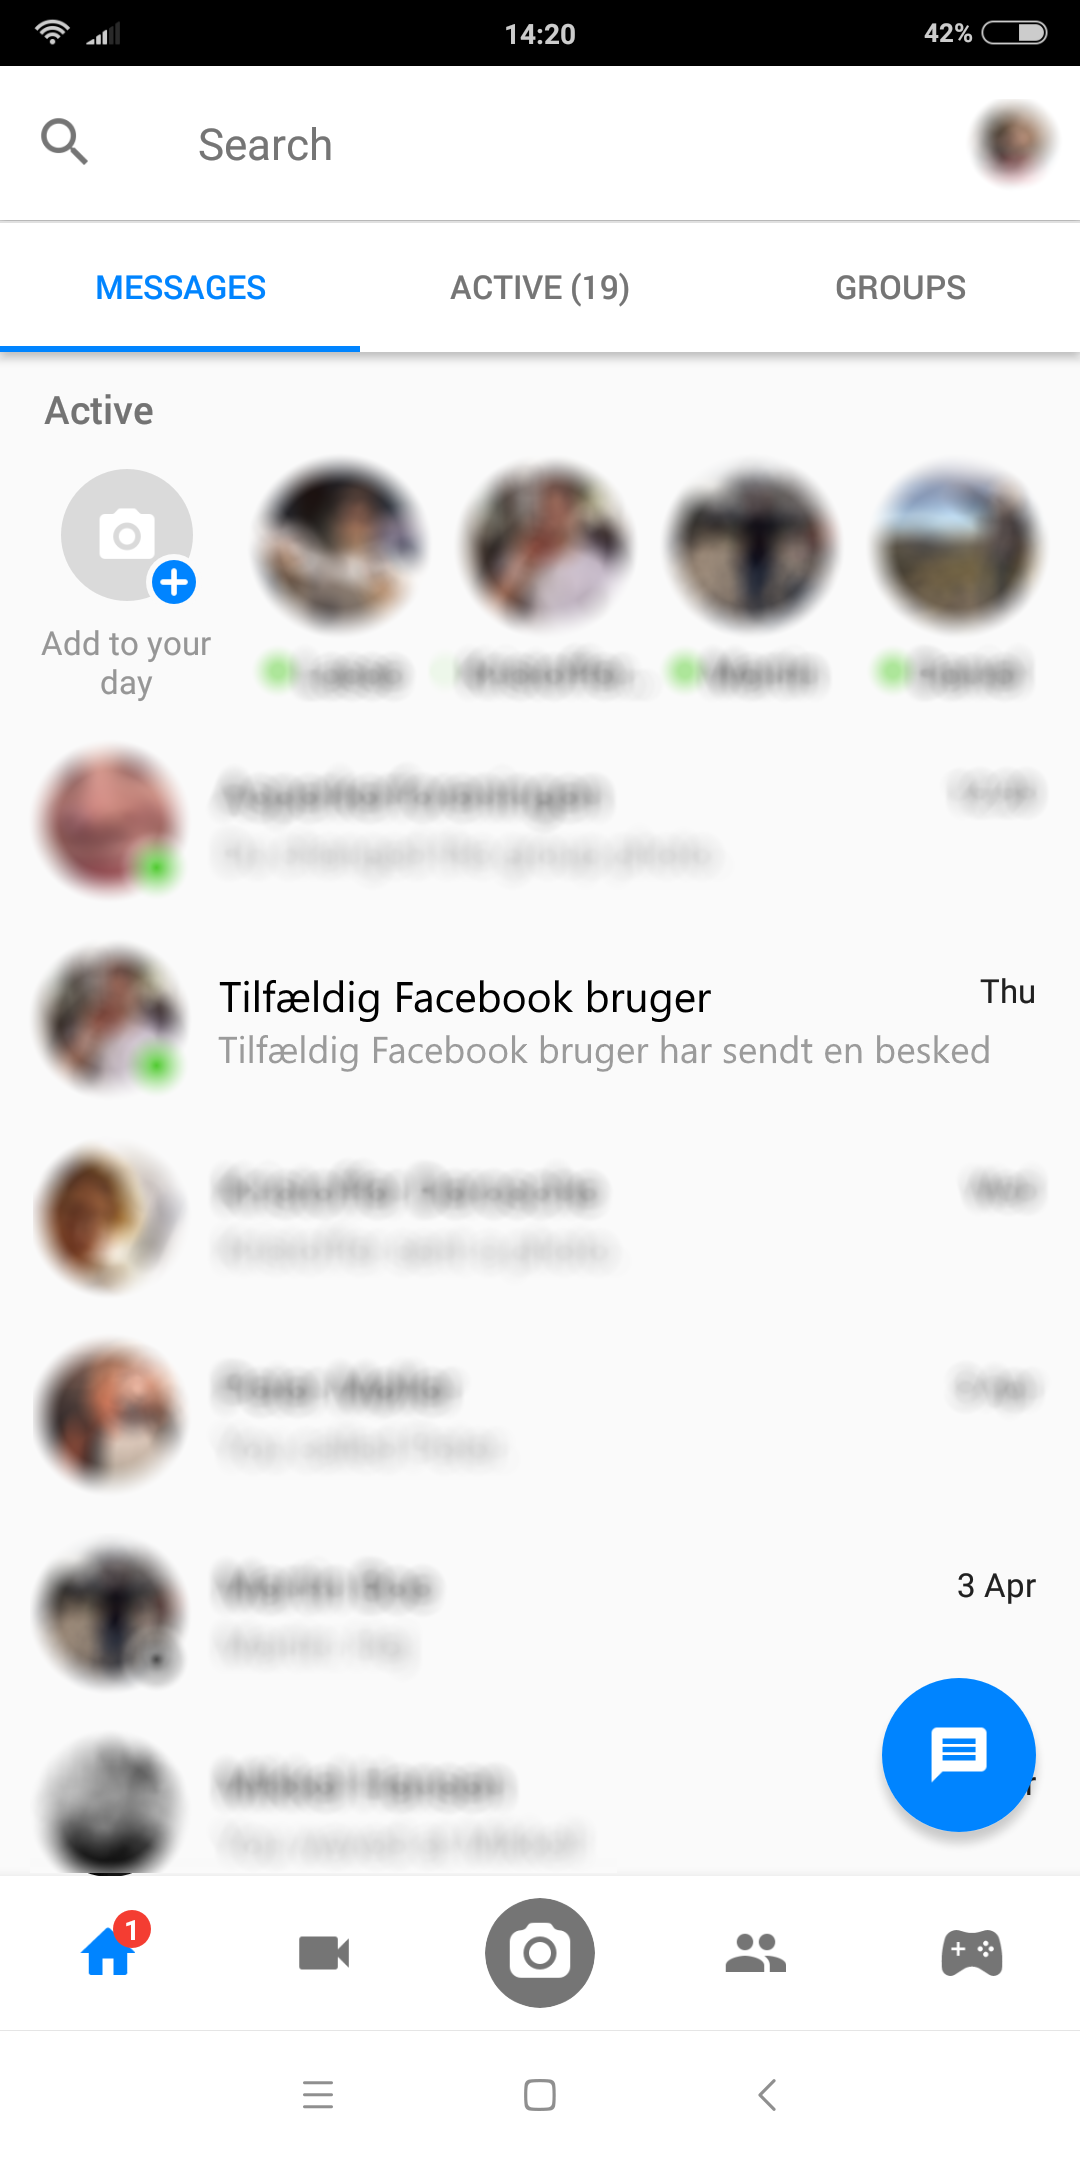
\includegraphics[scale=0.15]{Projectdoc/Problemanalyse/Illustrationer/1-fbchat.png} 
        \caption{Facebook messenger hovedmenu med chathoveder}
        \label{fig:facebookchat1}
    \end{subfigure}
    \begin{subfigure}{0.33\textwidth}
        \centering
        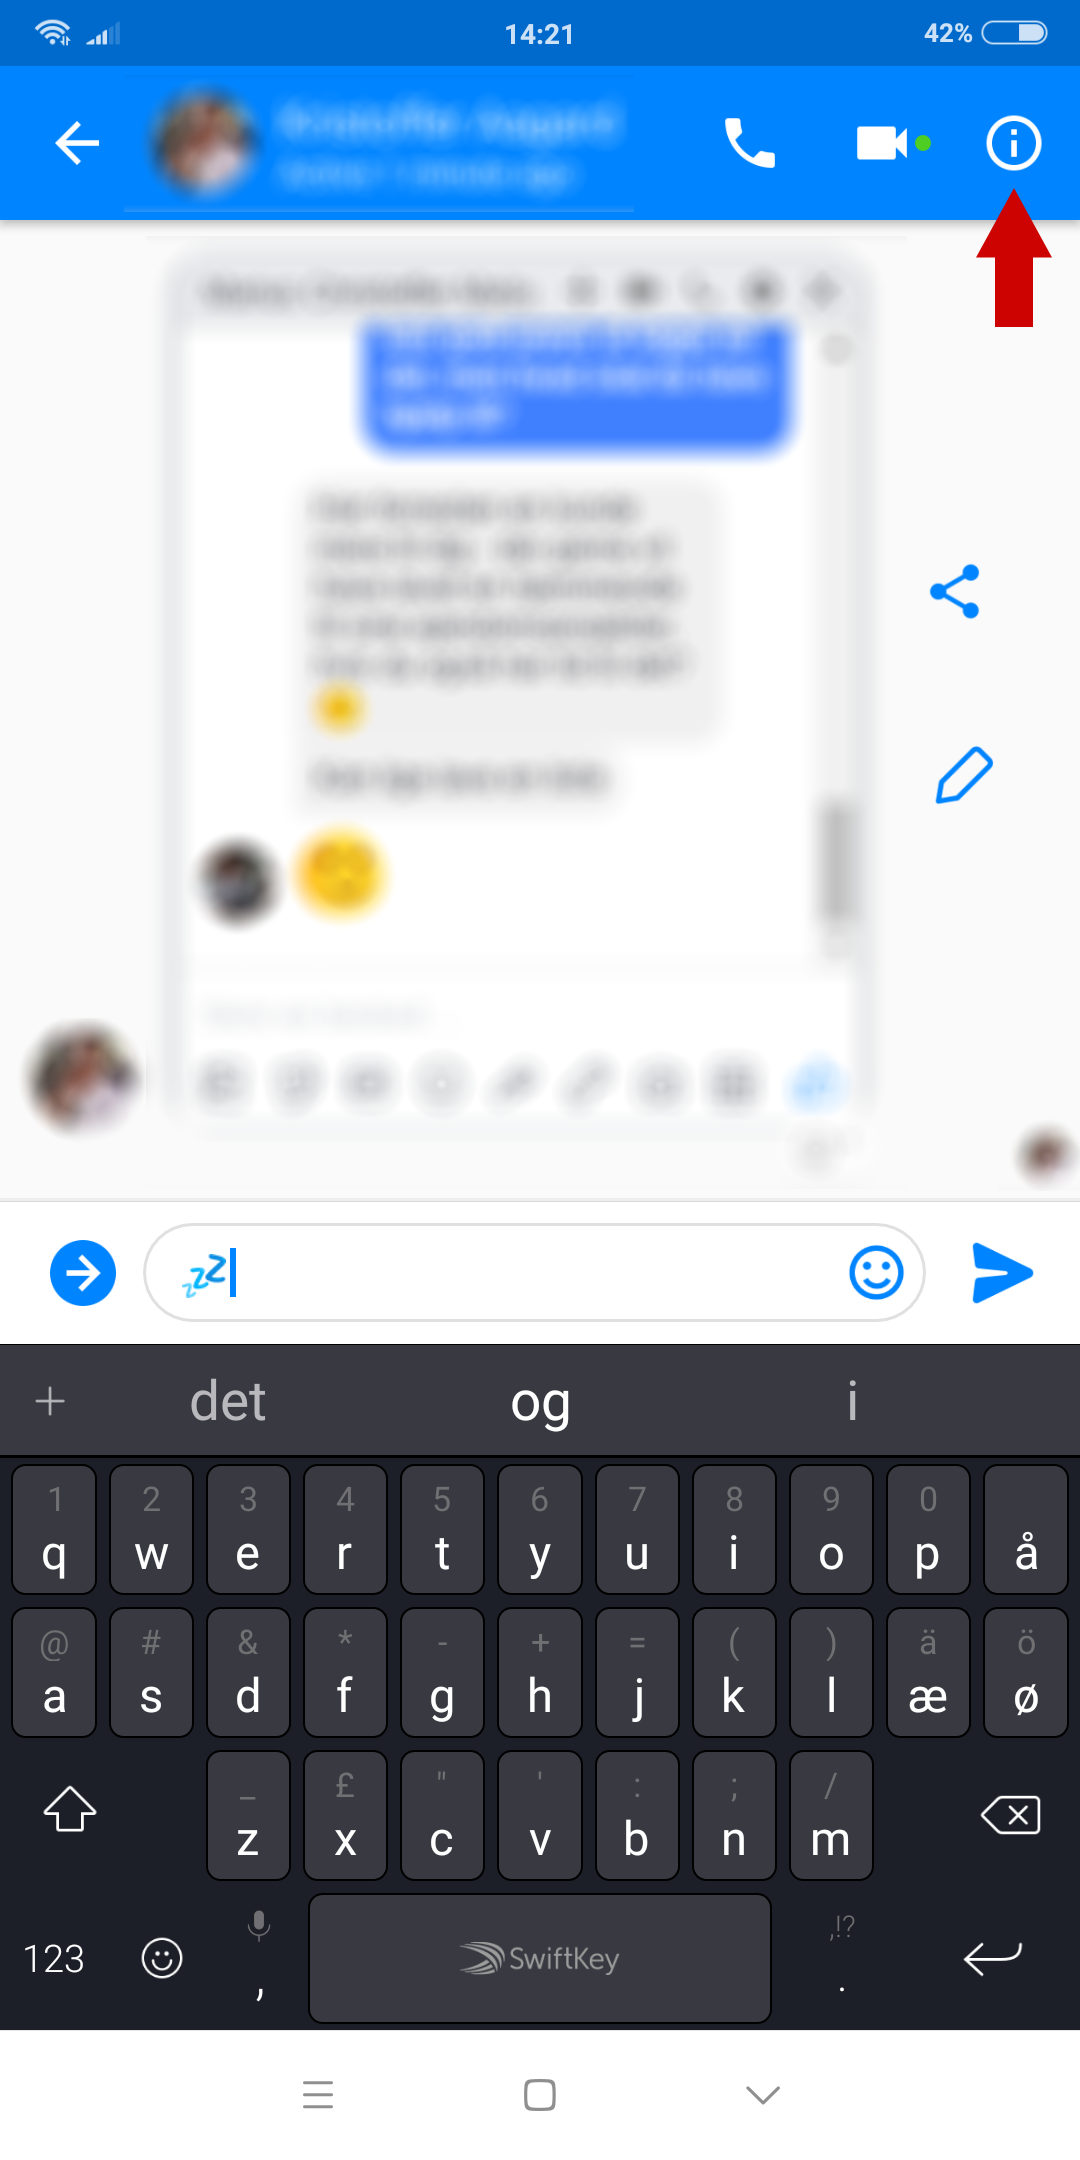
\includegraphics[scale=0.15]{Projectdoc/Problemanalyse/Illustrationer/2-fbchat.png}
        \caption{Indeni et standard ukrypteret privat chathoved}
        \label{fig:facebookchat2}
    \end{subfigure}
    \begin{subfigure}{0.33\textwidth}
        \centering
        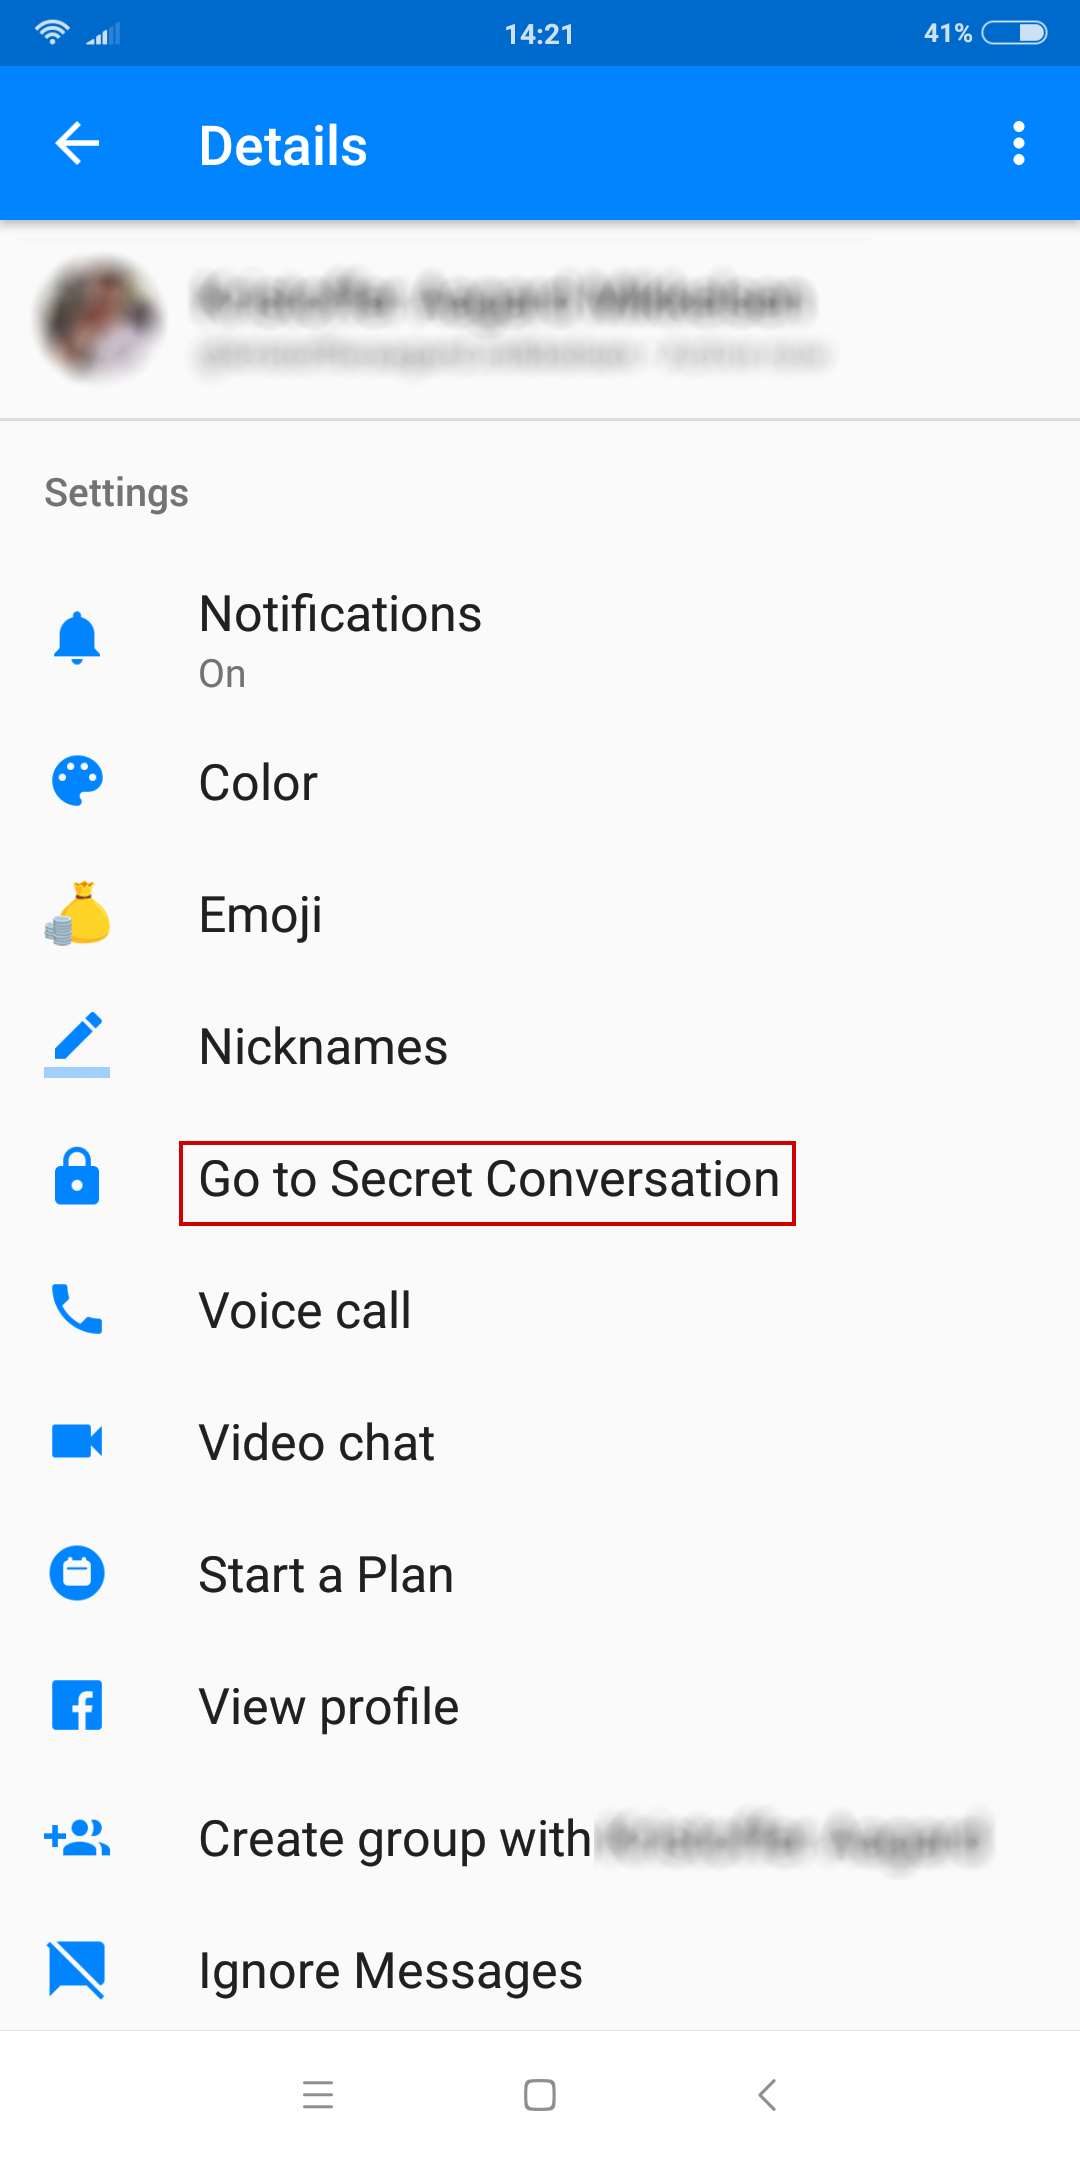
\includegraphics[scale=0.15]{Projectdoc/Problemanalyse/Illustrationer/3-fbchat.png} 
        \caption{Muligheden for "Hemmelig samtale" er opt-in i chathovedets indstillinger}
        \label{fig:facebookchat3}
    \end{subfigure}
    \begin{center}
        \begin{subfigure}{0.33\textwidth}
            \centering
            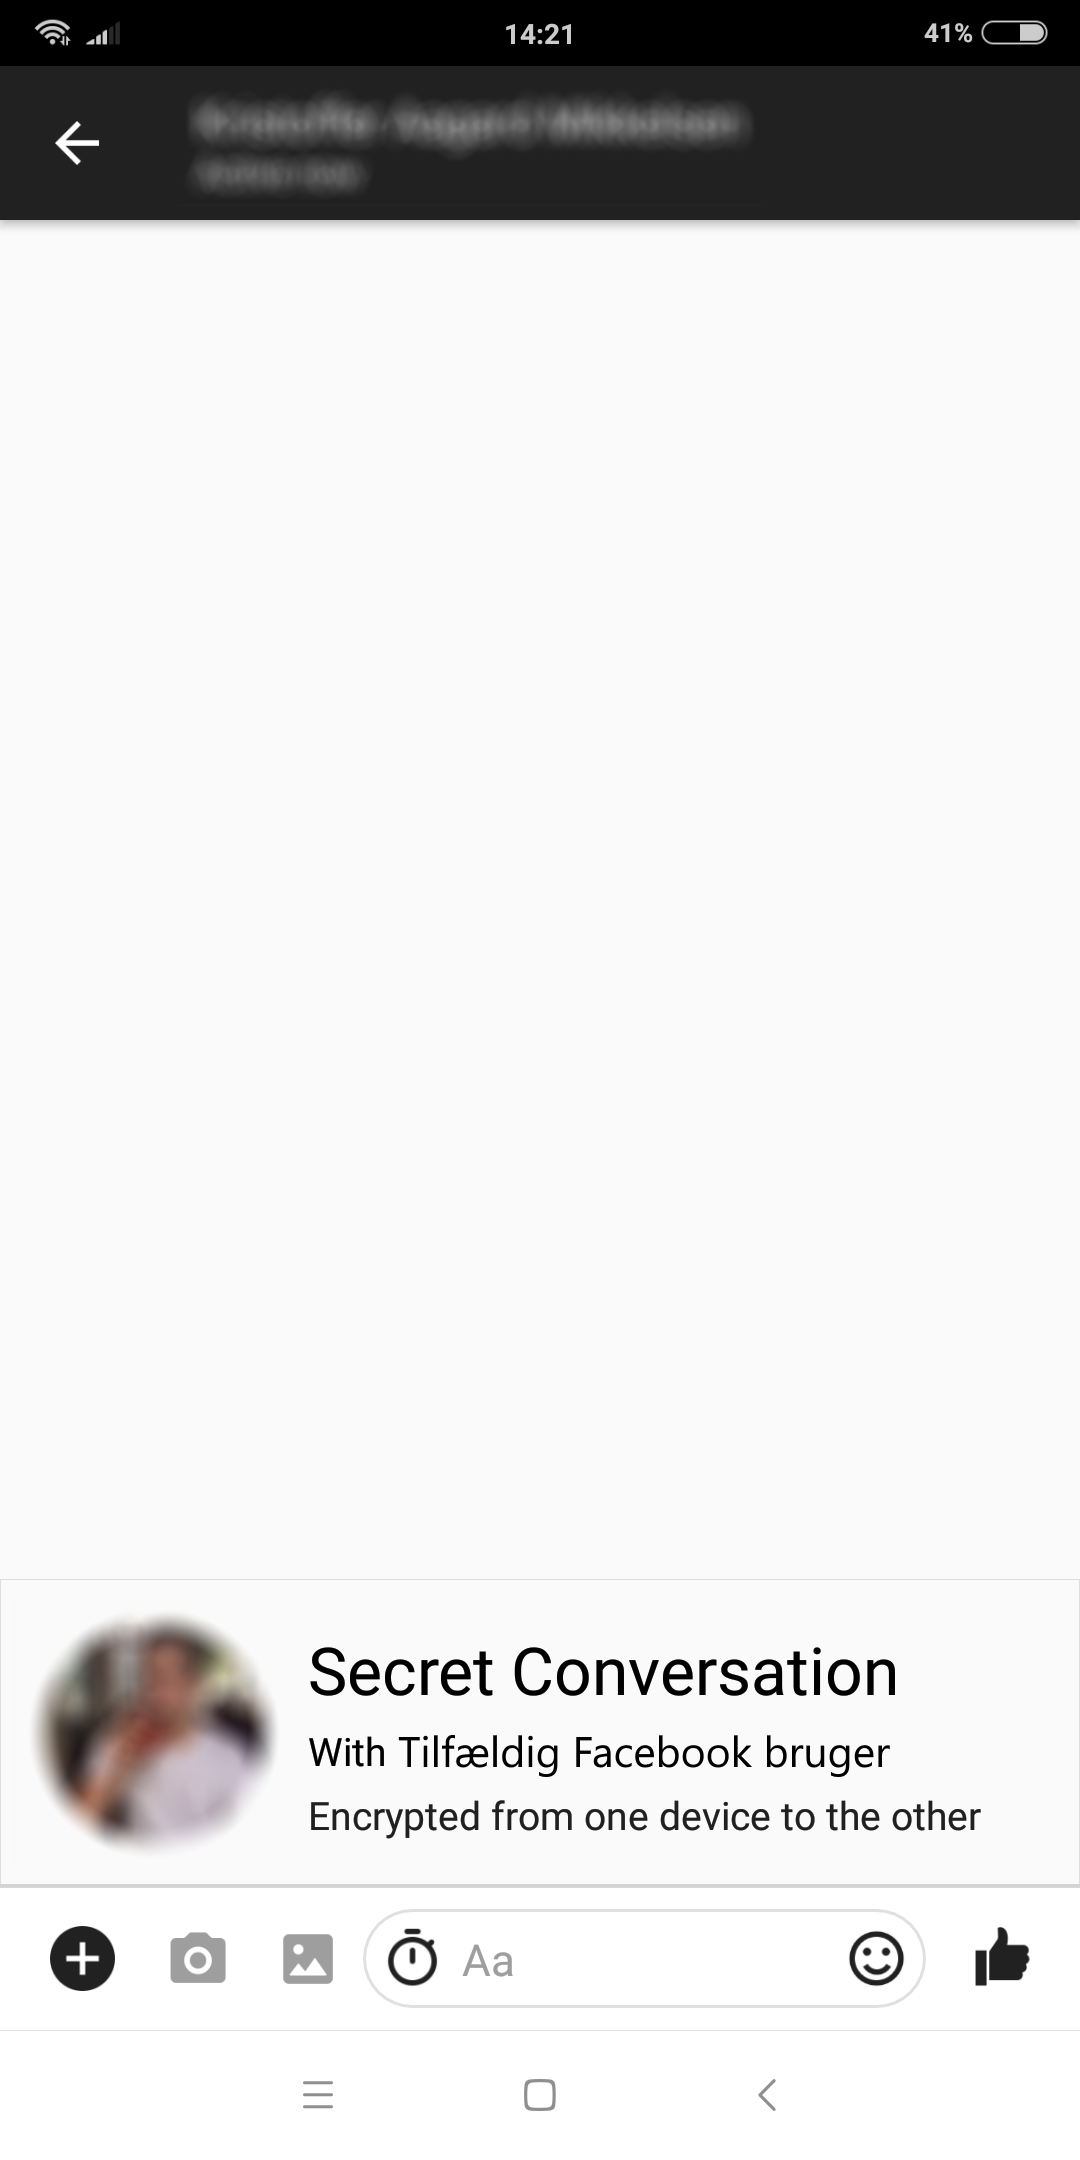
\includegraphics[scale=0.15]{Projectdoc/Problemanalyse/Illustrationer/4-fbchat.png} 
            \caption{Indeni et nyt separat chathoved til "Hemmelig samtale"}
            \label{fig:facebookchat4}
        \end{subfigure}
        \begin{subfigure}{0.33\textwidth}
            \centering
            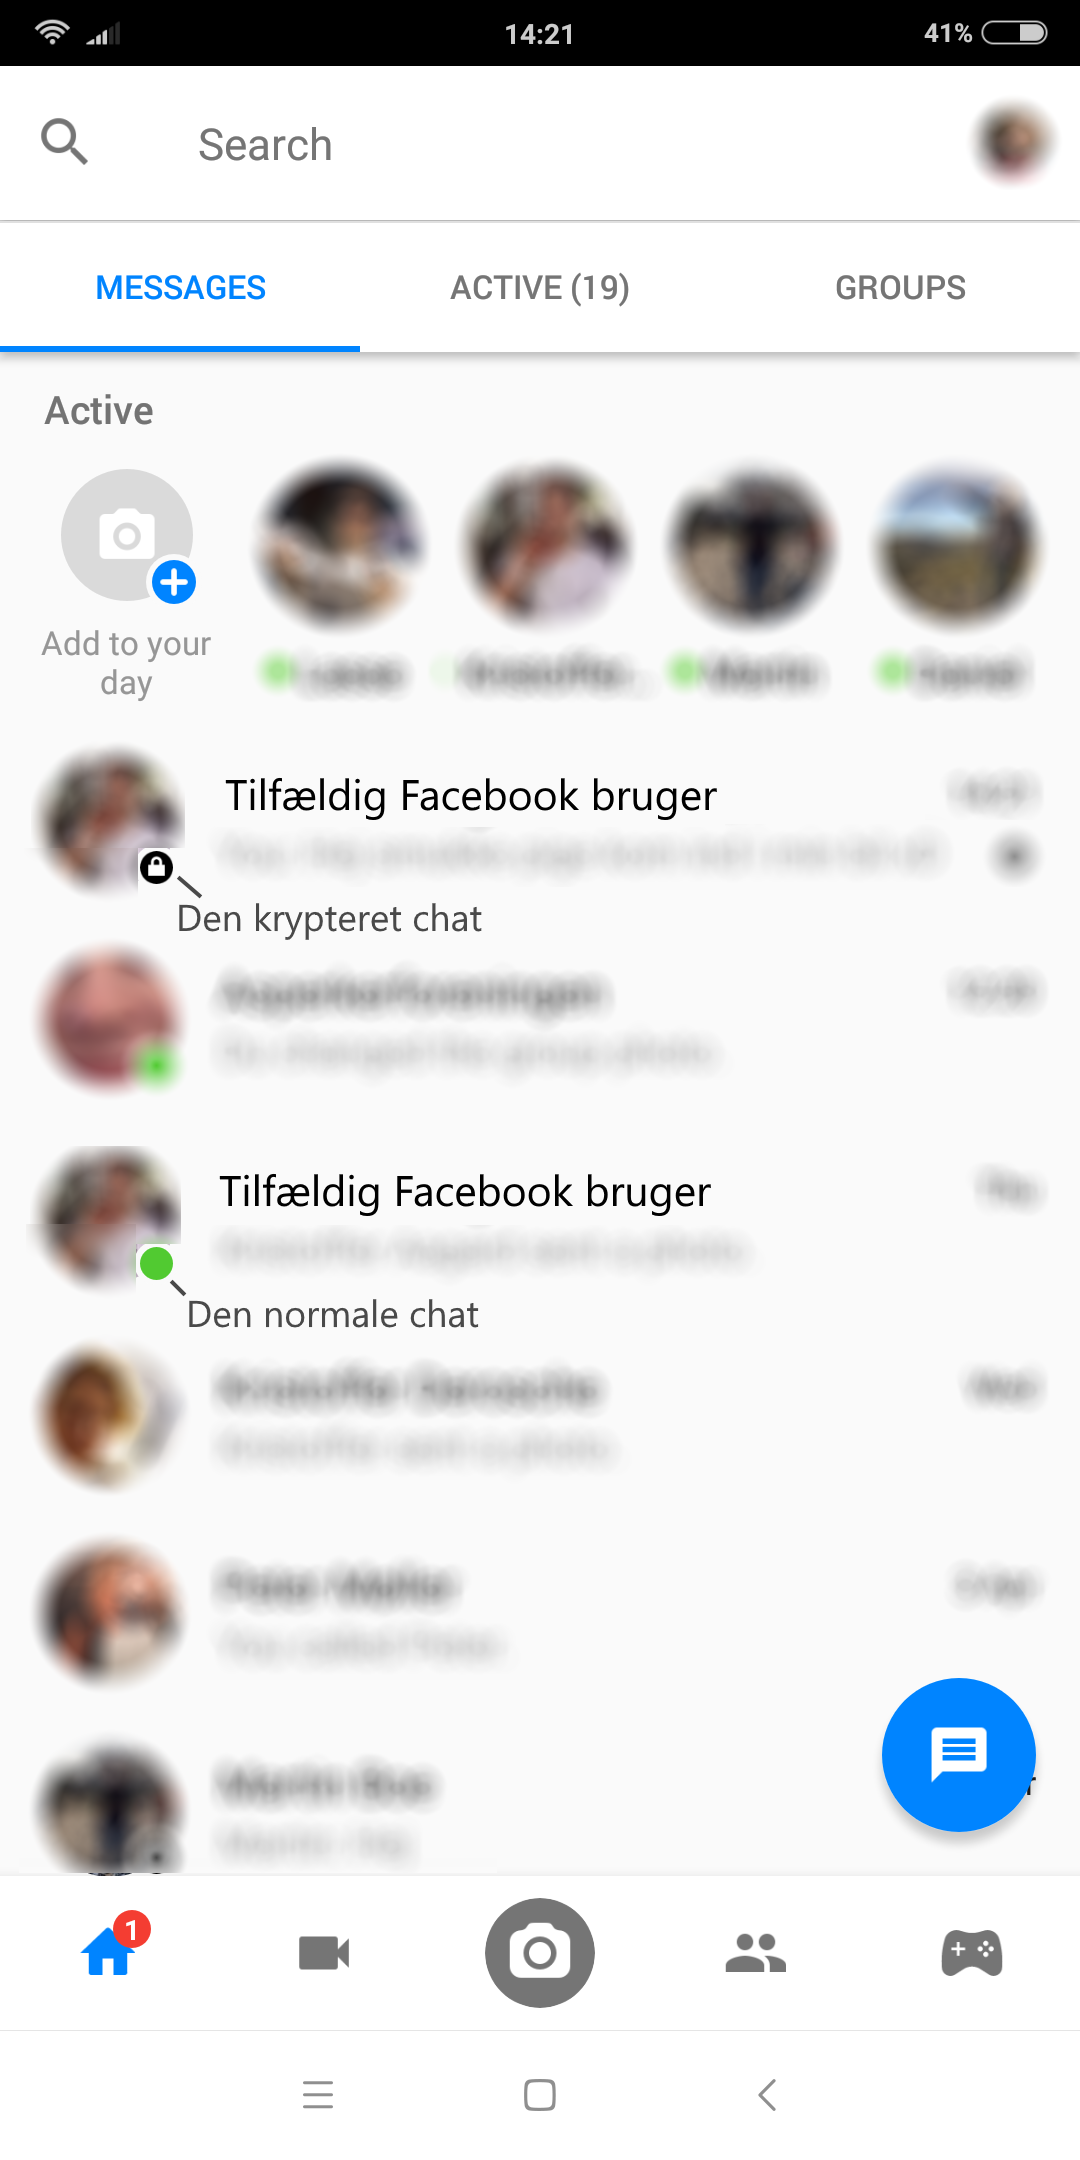
\includegraphics[scale=0.15]{Projectdoc/Problemanalyse/Illustrationer/5-fbchat.png} 
            \caption{Her ses hvordan det hemmelige chathoved og standard chathoved eksister hver for sig i oversigten}
            \label{fig:facebookchat5}
        \end{subfigure}
    \end{center}
    \caption{Facebook messengers forløb for at aktivere en "Hemmelig samtale"}
    \label{fig:facebookchat}
\end{figure}
